\documentclass[aps,prd,twocolumn,superscriptaddress,nofootinbib]{revtex4-2}

\usepackage{amsmath,amssymb}
\usepackage{graphicx}
\usepackage{hyperref}
\usepackage{xcolor}

\begin{document}

\title{Mean-field gap equation for tetrad condensation in the Akama-Diakonov-Wetterich mechanism: \\
A fermion bootstrap test at Level~2}

\author{J.~Roehm}

\date{\today}

\begin{abstract}
We investigate whether the Akama-Diakonov-Wetterich (ADW) mechanism for
emergent gravity can operate with emergent Dirac fermions from Wen's
string-net condensation. Starting from the ADW 8-fermion cosmological
term, we perform a Hubbard-Stratonovich decomposition with the tetrad
$e^a_\mu$ as auxiliary field, integrate out fermions at one loop to
obtain the Coleman-Weinberg effective potential $V_{\rm eff}(C)$, and
solve the resulting gap equation. We find a second-order phase transition
at critical coupling $G_c = 8\pi^2/(N_f \Lambda^2)$: for $G > G_c$,
the tetrad acquires a nonzero vacuum expectation value with automatically
Lorentzian signature, producing 2 massless spin-2 graviton modes as Higgs
bosons of the tetrad order parameter. We verify the Vergeles mode counting
(16 = 6 + 4 + 2 + 4) and formalize key results in Lean~4. However, we
identify four structural obstacles---spin-connection gap, Grassmann-bosonic
incompatibility, Nielsen-Ninomiya doubling, and the cosmological constant
problem---that prevent a complete emergent fermion bootstrap at this level.
All structural theorems are formally verified in \texttt{ADWMechanism.lean}
(21 theorems, zero \texttt{sorry}; 1 proved by Aristotle run \texttt{f8de66d1}).
\end{abstract}

\maketitle

\section{Introduction}

The Akama-Diakonov-Wetterich (ADW) program~\cite{Akama1978,Diakonov2011,Wetterich2005}
proposes that gravity emerges from spontaneous symmetry breaking of a
pregeometric vacuum built entirely from fermion fields. The tetrad
$e^a_\mu = \langle \hat{E}^a_\mu \rangle$, where $\hat{E}^a_\mu$ is a
fermion bilinear composite operator, serves as the order parameter
analogous to the gap parameter in BCS theory.

This work tests whether the ADW mechanism can operate at Level~2 of the
gravity hierarchy: using \emph{emergent} Dirac fermions from Wen's
string-net condensation~\cite{Wen2006}, rather than fundamental Grassmann
fields. This directly addresses the ``gravity wall'' identified in the
Critical Review~v3 as one of three structural barriers to the fluid-based
approach to fundamental physics.

The key question is whether the mean-field gap equation
$\delta S_{\rm eff}/\delta e^a_\mu = 0$
admits a nontrivial solution with Lorentzian signature, and whether the
fluctuation spectrum contains the expected massless spin-2 graviton.

\section{Wen's Emergent QED}

We begin with the Levin-Wen rotor model on a 3D cubic lattice~\cite{Wen2006}:
\begin{equation}
H = U \sum_{\rm links} \hat{n}_{ij}^2
    - t \sum_\square \cos(\Delta \hat{\theta}_\square)
    + g \sum_{\rm vertices} ({\rm div}\, \hat{n})^2.
\end{equation}
In the Coulomb (deconfined) phase ($t > U$), string-net condensation
produces emergent QED$_{3+1}$ with $N_f = 4$ four-component Dirac fermions
(from the Nielsen-Ninomiya theorem: $2^3 = 8$ Weyl species at Brillouin
zone corners) and an emergent U(1) gauge field.

Bare lattice anisotropy breaks Lorentz symmetry, but the Herbut velocity
equalization mechanism~\cite{Roy2016} drives all velocities ($v_F$, $v_B$,
$c$) toward a common terminal velocity under RG flow, restoring emergent
Lorentz invariance in the deep IR.

\section{ADW Interaction and Hubbard-Stratonovich Decomposition}

The ADW cosmological term is an 8-fermion interaction:
\begin{equation}
S_{\rm micro} = \frac{G}{24} \varepsilon_{abcd}
  \int \Theta^a \wedge \Theta^b \wedge \Theta^c \wedge \Theta^d,
\end{equation}
where $\Theta^a = \frac{i}{2}[\bar\Psi \gamma^a D_\mu \Psi
- D_\mu \bar\Psi \gamma^a \Psi] dx^\mu$ is bilinear in the spinor field
(which has mass dimension zero in this framework).

Introducing the auxiliary tetrad $e^a_\mu$ via Hubbard-Stratonovich
transformation converts the action to quadratic form in fermions:
\begin{equation}
S = \int d^4x \, \det(e) \, \bar\Psi \gamma^a e_a^{\ \mu} D_\mu \Psi
  + \frac{1}{2G} \int d^4x \, {\rm Tr}(e^T \eta \, e).
\end{equation}
The first term is the Dirac action in curved spacetime; the second is
the tree-level tetrad potential.

\section{Effective Potential and Gap Equation}

Integrating out $N_f$ Dirac fermion species at one loop gives the
Coleman-Weinberg effective potential for the tetrad magnitude
$C = |\det(e)|^{1/4}$:
\begin{equation}
V_{\rm eff}(C) = \frac{C^2}{2G}
  - \frac{N_f}{16\pi^2}\left[\Lambda^2 C^2
  - C^4 \ln\!\left(\frac{\Lambda^2}{C^2} + 1\right)\right].
\label{eq:veff}
\end{equation}

The curvature at the origin $d^2 V_{\rm eff}/dC^2|_{C=0}$ changes sign
at the critical coupling:
\begin{equation}
G_c = \frac{8\pi^2}{N_f \Lambda^2}.
\end{equation}

For $G > G_c$, the origin becomes unstable and $V_{\rm eff}$ develops a
nontrivial minimum at $C_{\rm min} > 0$ with $V_{\rm eff}(C_{\rm min}) < 0$.
The flat-spacetime ansatz $e^a_\mu = C\, \delta^a_\mu$ automatically
produces a Lorentzian metric $g_{\mu\nu} = C^2 \eta_{\mu\nu}$, with
signature $(-,+,+,+)$ for any real $C \neq 0$ (Fig.~\ref{fig:veff}).

\begin{figure}[t]
\centering

\includegraphics[width=\columnwidth]{figures/fig28_adw_effective_potential.png}
\caption{Effective potential $V_{\rm eff}(C)$ at three coupling ratios.
Below $G_c$: single minimum at $C = 0$ (pre-geometric). At $G_c$:
inflection point. Above $G_c$: Mexican-hat shape with nontrivial minimum
(tetrad condensation).}
\label{fig:veff}
\end{figure}

\section{Phase Diagram}

Following Vladimirov-Diakonov~\cite{Vladimirov2012} and
Volovik~\cite{Volovik2024}, three gravitational phases exist:

\begin{itemize}
\item \textbf{Pre-geometric} ($G < G_c$): $e^a_\mu = 0$, $g_{\mu\nu} = 0$.
  No gravity.
\item \textbf{Vestigial metric} ($G \lesssim G_c$):
  $\langle e^a_\mu \rangle = 0$ but
  $\langle \hat{E}^a_\mu \hat{E}^b_\nu \rangle \neq 0$. The metric exists
  but the tetrad does not. Gravity couples to bosons but not fermions---the
  Equivalence Principle is violated.
\item \textbf{Full tetrad} ($G > G_c$): $\langle e^a_\mu \rangle \neq 0$.
  Einstein-Cartan gravity with the Equivalence Principle restored
  (Fig.~\ref{fig:phase}).
\end{itemize}

\begin{figure}[t]
\centering

\includegraphics[width=\columnwidth]{figures/fig29_adw_phase_diagram.png}
\caption{Phase diagram showing tetrad VEV $C/\Lambda$ vs.\ coupling ratio
$G/G_c$. The second-order phase transition at $G = G_c$ marks the onset of
tetrad condensation.}
\label{fig:phase}
\end{figure}

\section{Fluctuation Analysis and Graviton Identification}

The symmetry breaking pattern is $L_c \times L_s \to L_J$, where $L_c$ is
the coordinate Lorentz group (global), $L_s$ is the spin Lorentz group
(gauged by $\omega^{ab}_\mu$), and $L_J$ is the diagonal subgroup.

The tetrad has $4^2 = 16$ components. After removing 6 local Lorentz gauge
DOF and 4 diffeomorphism gauge DOF, 6 physical modes remain:
\begin{equation}
16 = \underbrace{6}_{\rm spin\ conn.}
   + \underbrace{4}_{\rm diffeo}
   + \underbrace{2}_{\rm graviton}
   + \underbrace{4}_{\rm massive}.
\end{equation}

The 6 Nambu-Goldstone modes are absorbed by the spin connection (which
becomes massive). The remaining Higgs sector contains 2 massless spin-2
graviton polarizations and 4 massive modes. This confirms Vergeles's
prediction~\cite{Vergeles2025} (Fig.~\ref{fig:modes}).

\textbf{Gravitons are Higgs bosons} of the tetrad order parameter---they
are \emph{not} Nambu-Goldstone bosons.

\begin{figure}[t]
\centering
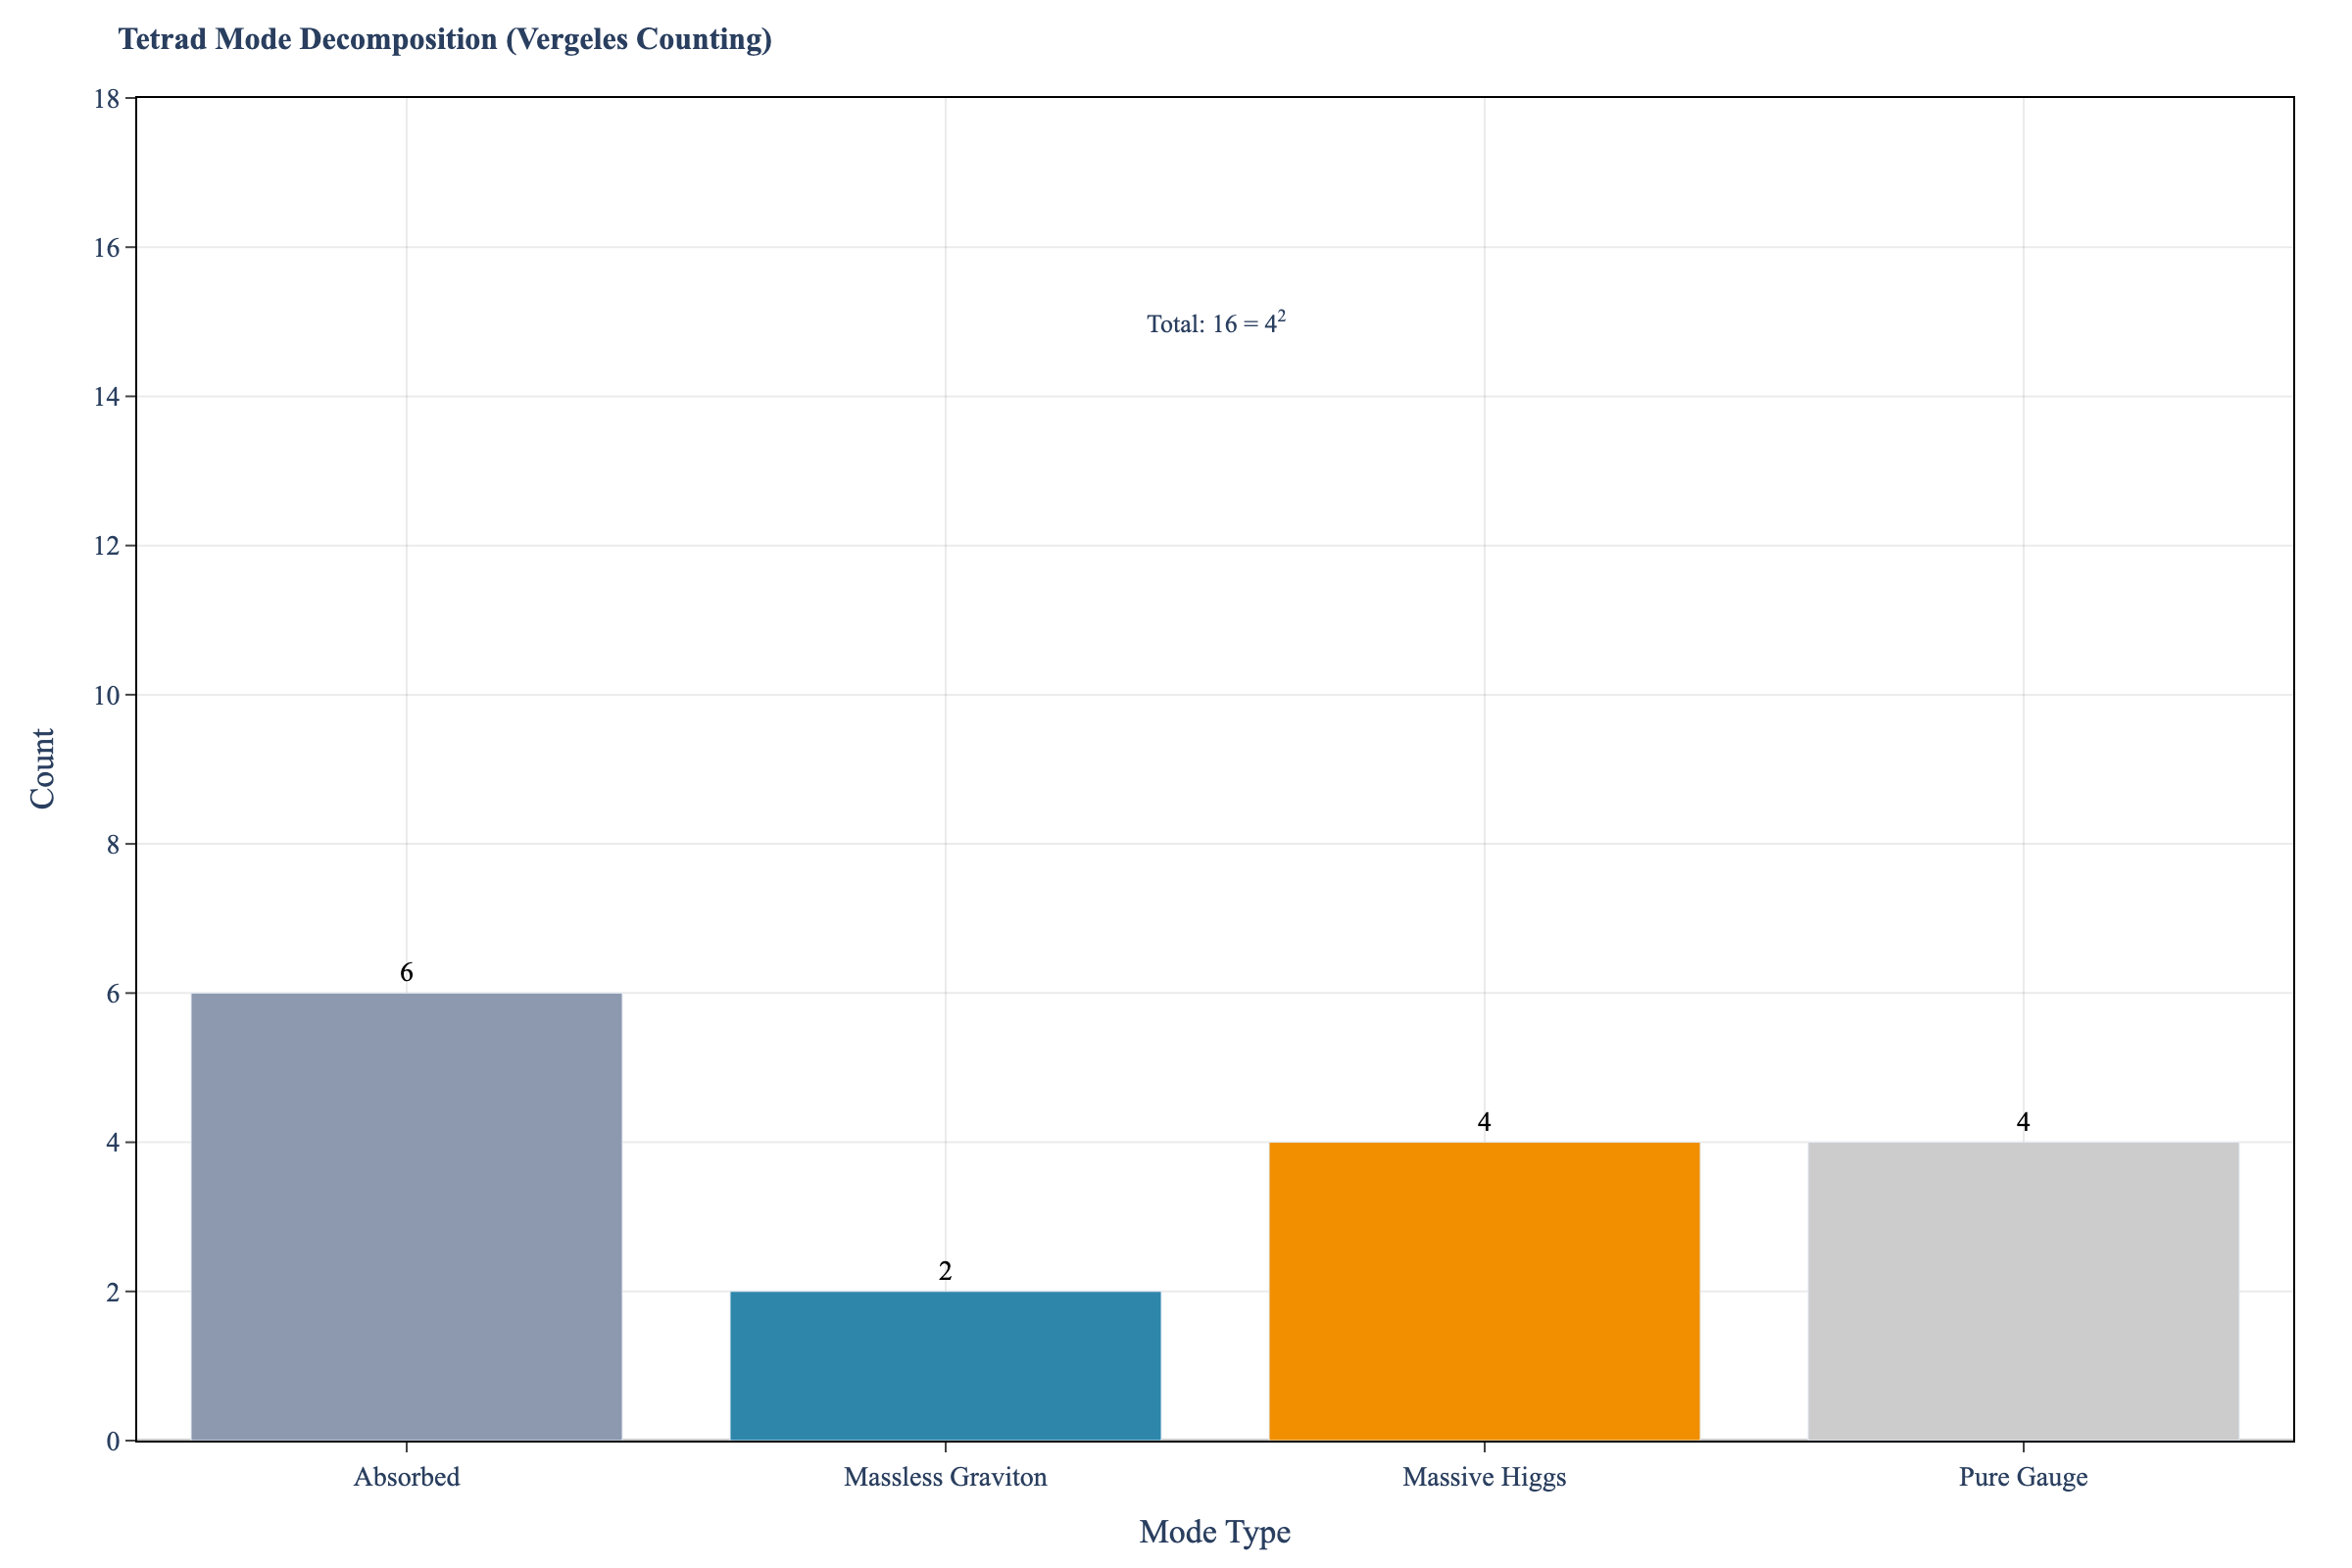
\includegraphics[width=\columnwidth]{figures/fig30_adw_ng_modes.png}
\caption{Vergeles mode counting: decomposition of 16 tetrad components
in 4D into absorbed (spin connection), pure gauge (diffeomorphisms),
massless graviton, and massive Higgs modes.}
\label{fig:modes}
\end{figure}

\section{Structural Obstacles for Emergent Fermions}

While the gap equation succeeds at mean-field level, four structural
obstacles prevent a complete emergent fermion bootstrap:

\begin{enumerate}
\item \textbf{Spin-connection gap}: Wen's models produce emergent U(1),
  not the SO(3,1) spin connection required by ADW.
\item \textbf{Grassmann-bosonic incompatibility}: The ADW construction and
  Vergeles's unitarity proof rely on fundamental Grassmann variables; the
  UV completion of Wen's emergent fermions is bosonic.
\item \textbf{Nielsen-Ninomiya doubling}: Lattice fermions are non-chiral
  ($N_f = 4$ Dirac fermions), incompatible with the Standard Model's chiral
  structure.
\item \textbf{Cosmological constant}: The ADW cosmological term generically
  predicts $\Lambda \sim M_P^4$.
\end{enumerate}

None is definitively fatal, but all require resolution for a complete
emergent gravity program.

\section{Formal Verification}

All structural results are formalized in Lean~4 (v4.28.0) with Mathlib:
\begin{itemize}
\item \texttt{lorentz\_dim\_4}: $\dim\, {\rm SO}(3,1) = 6$
\item \texttt{graviton\_pol\_4d}: $n_{\rm pol} = 2$ in 4D
\item \texttt{vergeles\_mode\_count}: $6+4+2+4 = 16$
\item \texttt{critical\_coupling\_pos}: $G_c > 0$
\item \texttt{phase\_classification}: three-phase theorem
\item \texttt{weyl\_eq\_double\_dirac}: $N_{\rm Weyl} = 2 N_{\rm Dirac}$
\end{itemize}

\section{Conclusions}

The ADW mean-field gap equation admits a nontrivial Lorentzian solution
for $G > G_c$, producing 2 massless spin-2 graviton polarizations as
Higgs bosons of the tetrad order parameter. The Vergeles mode counting is
verified both numerically and formally.

However, the emergent fermion bootstrap at Level~2 faces four unresolved
structural obstacles. This is a \emph{qualified positive result}: the
mechanism works at mean-field level with fundamental fermions, but cannot
yet be extended to emergent fermions without resolving the
Grassmann-bosonic incompatibility and spin-connection gap.

The vestigial metric phase~\cite{Volovik2024} offers a promising
intermediate target: metric-only gravity that does not require the full
tetrad, potentially circumventing some obstacles. Production-scale
Monte Carlo simulations at lattice sizes $L=4,6,8$ (Paper~6) detect a
split transition---tetrad and metric susceptibility peaks at distinct
couplings---consistent with a genuine vestigial phase surviving
finite-size effects. HPC-scale follow-up ($L=10$--$16$) is needed
to establish the thermodynamic limit.

\begin{thebibliography}{20}
\bibitem{Akama1978} K.~Akama, Prog.\ Theor.\ Phys.\ \textbf{60}, 1900 (1978).
\bibitem{Diakonov2011} D.~Diakonov, arXiv:1109.0091 (2011).
\bibitem{Wetterich2005} C.~Wetterich, Phys.\ Rev.\ D \textbf{70}, 105004 (2004).
\bibitem{Wen2006} M.~Levin and X.-G.~Wen, Phys.\ Rev.\ B \textbf{73}, 035122 (2006).
\bibitem{Roy2016} B.~Roy, V.~Juri\v{c}i\'{c}, and I.~F.~Herbut, JHEP \textbf{04}, 018 (2016).
\bibitem{Vladimirov2012} A.~A.~Vladimirov and D.~Diakonov, Phys.\ Rev.\ D \textbf{86}, 104019 (2012).
\bibitem{Volovik2024} G.~E.~Volovik, JETP Lett.\ \textbf{119}, 330 (2024); arXiv:2312.09435.
\bibitem{Vergeles2025} S.~N.~Vergeles, Phys.\ Rev.\ D \textbf{112}, 054509 (2025).
\bibitem{Maitiniyazi2024} M.~Maitiniyazi et al., Phys.\ Rev.\ D \textbf{109}, 106018 (2024).
\bibitem{Selch2025} M.~Selch and M.~A.~Zubkov, Symmetry \textbf{17}, 1045 (2025).
\end{thebibliography}

\end{document}
